\section{面向开放组织的数据信息挖掘框架}
% 从Github全域数据中能提取到什么信息,即看板展现的内容。【数据结构】(这里要直接讲数据结构吗?】
% 意义:
% 快速挖掘出项目中的深层信息
% 帮助开源项目的管理
% 帮助个人职业规划与发展
\par 上一章中,对开源社区中开放数据的探索性分析从社区活跃情况、开源开发者的工作时间分布、开发语言的使用、项目或开发者之间的协同关系四个角度,带来了对项目或个人开发者行为的更深层解读,揭露了开源社区庞大的开放数据中所含信息量的冰山一角。如果这些信息能够被快速挖掘、定向展现,那么将大大助益开源社区的发展。

\par 对于开源开发者而言,通过个人行为数据的汇总挖掘,能够更好地自我了解与进行职业规划;对于开源项目而言,这些数据将提供不同的维度来评估其影响力、国际化程度,即便对于项目不熟悉的人,也能在很短的时间内快速了解项目状况,更可以方便项目管理与社区治理。


\subsection{衡量指标定义}
% 活跃仓库与开发者统计方法;
% ​开发者活跃度;
% ​项目活跃度;
% 时区估计方法;
% 主要开发语言;
% ​开发者协作网络构建方法;
\subsubsection{活跃仓库与开发者统计方法}
\par 若被统计的代码仓库包含事件日志,仓库即被定义为活跃仓库;若开发者有任意代码仓库包含事件日志,开发者即被定义为活跃开发者。

\subsubsection{开发者活跃度}
\par 开发者活跃度,其定义为某特定 GitHub 账号在一段时间内在某特定 GitHub 项目中的活跃评价指标。其活跃度由该账号在该项目中的行为数据决定,本报告中所关心的行为包含如下几种:

\begin{itemize}
    \item Issue comment:在 issue 中参与讨论是最基本的行为,每个评论计入 1 次。
    \item Open issue:在项目中发起一个 issue,无论是讨论、bug 报告或提问,对项目都是带来活跃的,每个发起的 issue 计入 1 次。
    \item Open pull request:为项目提交一个 PR,表示已对该项目进行源码贡献,则每次发起一个 PR 计入 1 次。
    \item Pull request review comment:对项目中的 PR 进行 review 和讨论,需要对项目有相当的了解,并且对项目源码的质量有极大帮助,每个评论计入 1 次。\\
          注:仅通过代码 review 对特定代码行的讨论记为 review,直接对 PR 的评论回复记为 issue comment 事件。
    \item Pull request merged:若有 PR 被项目合入,即便是很小的改动,也需要对项目有较为深入的理解,是帮助项目进步的真切贡献,则每有一个 PR 被合入计入 1 次,同时 PR 合入事件根据该 PR 的代码增加行数。
    \item Watch:用户 star 项目,被计入 1 次。注:Star 操作在 GitHub 日志事件中记为 Watch 事件。
    \item Fork:开发者 fork 该项目,被计入 1 次。
\end{itemize}
% //TODO: 寻找参考文献
以上 7 个种行为在该报告模型中各自独立计数,具有不一样的权重,根据专家经验,加权值分别为 1、2、3、4、2,1,2,即:
$$
 A_{u\_d}=C_{issue\_comment}+2{C}_{open\_issue}+3{C}_{open\_pr}+4{C}_{review\_comment}+2{C}_{pr\_merged}+{C}_{watch}+2{C}_{fork} 
$$
其中,Pull request merged 的计数由分段函数决定:

$$ C_{pr\_merged}=\left\{
    \begin{array}{rcl}
        0.8+0.002 \times loc &  & {loc < 100}          \\
        1                    &  & {100 \leq loc < 300} \\
        2.5-0.005 \times loc &  & {300 \leq loc < 400} \\
        0.5                  &  & {loc \geq 400}
    \end{array} \right.
$$

其中,loc 表示新增的代码行数。根据软件计量学经典数据统计,单次代码变更最佳在 200 行以内,超过 400 行的代码变更会导致审阅困难,故通过分段函数关联了代码新增行数与 PR 的权重指标。

\subsubsection{项目活跃度}
\par 项目活跃度定义为某特定项目在一段时间内的活跃评价指标。其活跃度由单开发者在一天内的活跃度加总计算得到(时间点与时间段计算方式均基于开发者个人活跃度方式计算):

$$ A_{r} = \sum (A_{u\_d} / day\_count) $$

开发者活跃仓库数量,则在此基础上定义为,由每个开发者所产生的活跃度大于 0 的仓库数量。

\subsubsection{开发者时区估计方法}

\par 根据开发者全年每小时产生日志的数量,计算获取其事件最多的连续 12 个小时,令其时间为该开发者本地时间的 9 时至 21 时,则可以大致确定该开发者的所属时区。因为日志所记录的时间为 UTC 标准时间\footnote{
UTC 即协调世界时间,是国际通用的时间标准,将全球各地的时间进行同步协调。UTC 时间是经过平均太阳时(以格林威治时间 GMT 为准)、地轴运动修正后的新时标以及以秒为单位的国际原子时进行综合精算而得到的。
世界时区使用 UTC 的正或负偏移量表示。最西端的时区使用 UTC-12,比UTC落后十二小时;最东部的时区使用 UTC+14,比 UTC 早 14 小时。出现 UTC+13,UTC+14 的原因如下:
    \begin{enumerate}
        \item[1)] 因为国际日期变更线,虽然1884年划定时避免在一个国家中同时存在着两种日期,但是1979年成立的基里巴斯领土却跨越了国际日期变更线。基里巴斯的UTC有:莱恩群岛(UTC+14)、菲尼克斯群岛(UTC+13)、吉尔伯特群岛(UTC+12),这样保证一个国家内的日期为同一天。
        \item[2)] 因为夏令时,即天亮早的夏季人为将时间调快一小时。比如新西兰是 UTC+12,在夏时制改用 UTC+13。
    \end{enumerate}
北京时间是中国采用国际时区东八时区的区时作为标准时间,东八区(UTC+8)是比 UTC 早 8 小时的时区。
}。考虑开发者一天连续 12 个小时产生日志数最多的最后一个小时,其最后一小时(即本地时间 21 时)对应的 UTC 时间记为 $ k $, 则时区计算公式如下:
$$
    zone=
    \begin{cases}
        20-k^*, & k^*>8 \quad \text{对应本地为东时区}     \\
        -4-k^*, & k^*\le 8  \quad \text{对应本地为西时区}
    \end{cases}
$$

\par 其中,数学公式: $ k^*=argmax\{\sum_{i=k-11}^{k}{c_i} \},\quad  k=0,1,...,23 $, $ c_i $表示当前小时产生的日志数量。当 i 为负值时,意味着为前一天的时间,需进行转换,即使用数学公式: $ i=i+24 $进行转换。

\par 因单个开发者的行为具有偶发性与特殊性,本方法不可用于单开发者时区的精确估计,但其在统计维度上具有意义,在此仅考虑统计学意义。再者,活跃度较低的开发者,其行为发生也具有偶发特性,所以在对开发者时区判断时,剔除了 GitHub Apps 并只保留全域活跃度排名前 5 万名的开发者账号用于分析,得到的工作时间画像如图2-3所示。

\begin{figure}[H]
    \centering
    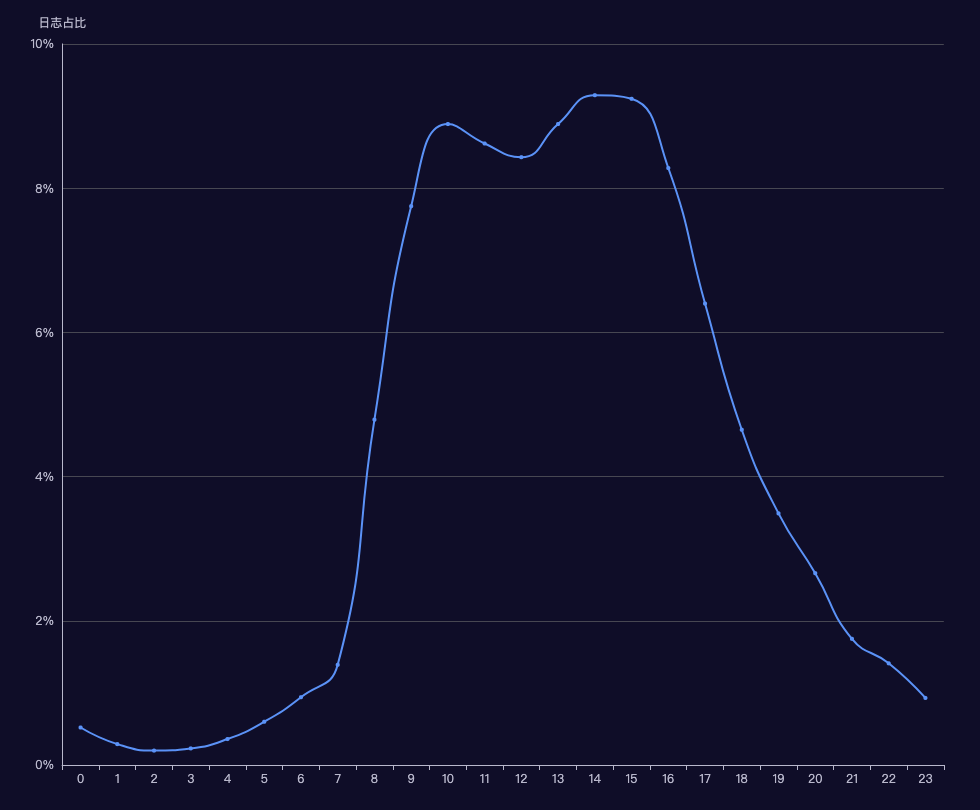
\includegraphics[width=130mm]{./figures/image2-3.png}
    \caption{ 典型开源开发者工作时间画像\\Portrait of a typical open source developer's working hours}
\end{figure}

\par 由图2-3所示,开发者通常会选择从当地时间早上 8 时开始工作,中午 11 - 13 时进行短暂的午休,随后在下午 15 - 16 时达到一个生产力高峰,并持续产出到晚间,较符合常见的工作时间情况;另一方面,可以看到开发者在晚间的工作产出比例还是较高的,甚至可以工作到凌晨 1 点,活跃程度应该明显高于一般职业。

\par 在高活跃开发者中,UTC-8 至 UTC-3,即美洲(美国、加拿大、南美)开发者分布最多,虽然单时区的开发者比例不是最高,但总体开发者占比高达 33\% 左右。而 UTC+1 至 UTC+3,即欧洲拥有最高的单时区开发者比例,UTC+1 时区高达近 10\%,三个时区的总占比约为 26\% 左右。总体而言,亚洲的开发者数量依然较少,但在 UTC+7 至 UTC+8 区域有一个小的波峰,说明中国、俄罗斯开发者相较其他国家还是有较高的开源活跃。而太平洋地区(UTC+9 至 UTC-9)则由于人口分布原因,开发者比例最低。


\subsubsection{开发者使用语言统计方法}
\par 开发者使用语言定义为一个开发者账号在该年度使用频率最高的语言,其具体实现为一个开发者账号在该年度提交并合入 PR 最多的项目所使用的主要编程语言。


\subsubsection{​开发者协作网络构建方法}
开发者协作网络是基于说明 2.1 中开发者活跃度的定义,通过多个开发者在项目中的协作关系进行构建的。具体构建过程为将每个开发者的全年活跃度计算精细化到具体的 issue/PR 之上,则同时在同一个 issue/PR 上有过活跃的开发者认为其具有协作关系,而协作关系与两人在该 issue/PR 上的活跃度相关,具体计算方式为:

$$ R_{ab}=\sum_{i}{\frac{A_{ia}A_{ib}}{A_{ia}+A_{ib}}} $$

其中 $ A_{ia}, A_{ib} $分别为开发者 a 和 b 在 issue/PR i 上的活跃度,计算方法遵循说明 2.1 中的活跃度计算方法,数学公式: $ R_{ab} $为开发者 a 和 b 在该项目上的协作关联度。即两个开发者在项目的协作关联度为其在所有共同活跃的 issue/PR 上的活跃度的调和平均值之和。该构建方式与 OpenGalaxy 的项目协作网络构建方式类似。


% \subsection{数据设计}
% 3.1~3.7中每个图表的形式、横纵轴【可视化方式】

% 指标列表与展示形式
% Project Activation(项目活跃度):项目在一段时间内的活跃度指标。具体计算方式由 Hypertrons 指定。
% 展示形式:折线图。横坐标:时间;纵坐标:活跃度。
% 示例:(注:下图表示的是多个项目的项目活跃度趋势对比图)
% 	图片: https://uploader.shimo.im/f/VWxActLXo2jKqwDW.png

% Project Attention (项目关注度):项目在一段时间内的关注度指标。具体计算方式由 Hypertrons 指定。
% 展示形式:折线图。横坐标:时间;纵坐标:关注度。
% 示例:(注:下图表示的是多个项目的项目关注度趋势对比图)
% 	图片: https://uploader.shimo.im/f/D196emAriigefDUX.png

% Number of Issues: 项目在一段时间内处于打开与关闭状态的 Issue 数量。
% 展示形式:条形图。横坐标:时间;y轴正轴:一段时间内创建的 Issue 数量;y轴负轴:一段时间内解决的 Issue 数量。
% 示例:
% 	图片: https://uploader.shimo.im/f/BzGOk956hRcEZUEy.png

% Number of Pull Request: 项目在一段时间内处于打开与关闭状态的 PR 数量。
% 展示形式:条形图。横坐标:时间;y轴正轴:一段时间内创建的 PR 数量;y轴负轴:一段时间内解决的 PR 数量。
% 示例:
% 	图片: https://uploader.shimo.im/f/ZW58nNK82S4DG9rE.png

% Number of Contributors:项目中一定时间段内贡献者数量。具体计算方式由 Hypertrons 指定。
% 展示形式:折线图。横坐标:时间;纵坐标:一段时间内的贡献者数量。
% 示例:
% 	图片: https://uploader.shimo.im/f/5pV3tvY8mBfhVDhW.png   
% Top N Contributors: 项目中累计活跃度排名前 N 名开发者。具体计算方式由 Hypertrons 指定。
% 展示形式:列表。
% 字段1:排名
% 字段2;活跃度。
% 示例:
% 	图片: https://uploader.shimo.im/f/3BFDAOGVKBffmNe1.png

% 嵌入位置
% GitHub
% 选项1:通过悬浮球,弹出新页面。(图待补充)
% 问题:
% 选项2:Repo 首页。如下图。
% 问题:指标项多的情况下,太长。
% 	图片: https://uploader.shimo.im/f/QwAGN85cslGcEu5T.png
% 选项3:Insights 页面。如下图(该图待优化)
% 问题:只能在原有的选项卡添加内容,无法做到:添加一个选项卡,并支持点击跳转。(待评估)
% 图片: https://uploader.shimo.im/f/v5aJqDAEOwA66kZ4.png

\subsection{开发者分析方法}
\subsubsection{个人活动}
% 开发者活跃度;
% 工作时间分布;
% ​Github事件雷达图;

% //TODO: 能否直接使用开源年报的图片?or标注出处?
\par 经统计,2020年GitHub 全域活跃项目数量约 5,421 万个,活跃开发者账号约 1,454 万,分别较 2019 年增长 36.4\% 与 21.8\%。通过对全域开发者进行活跃度与活跃仓库数量的统计,可以得到 GitHub 全域开发者的活跃度分布情况和单个开发者活跃仓库数量分布情况如下:
\begin{figure}[H]
    \centering
    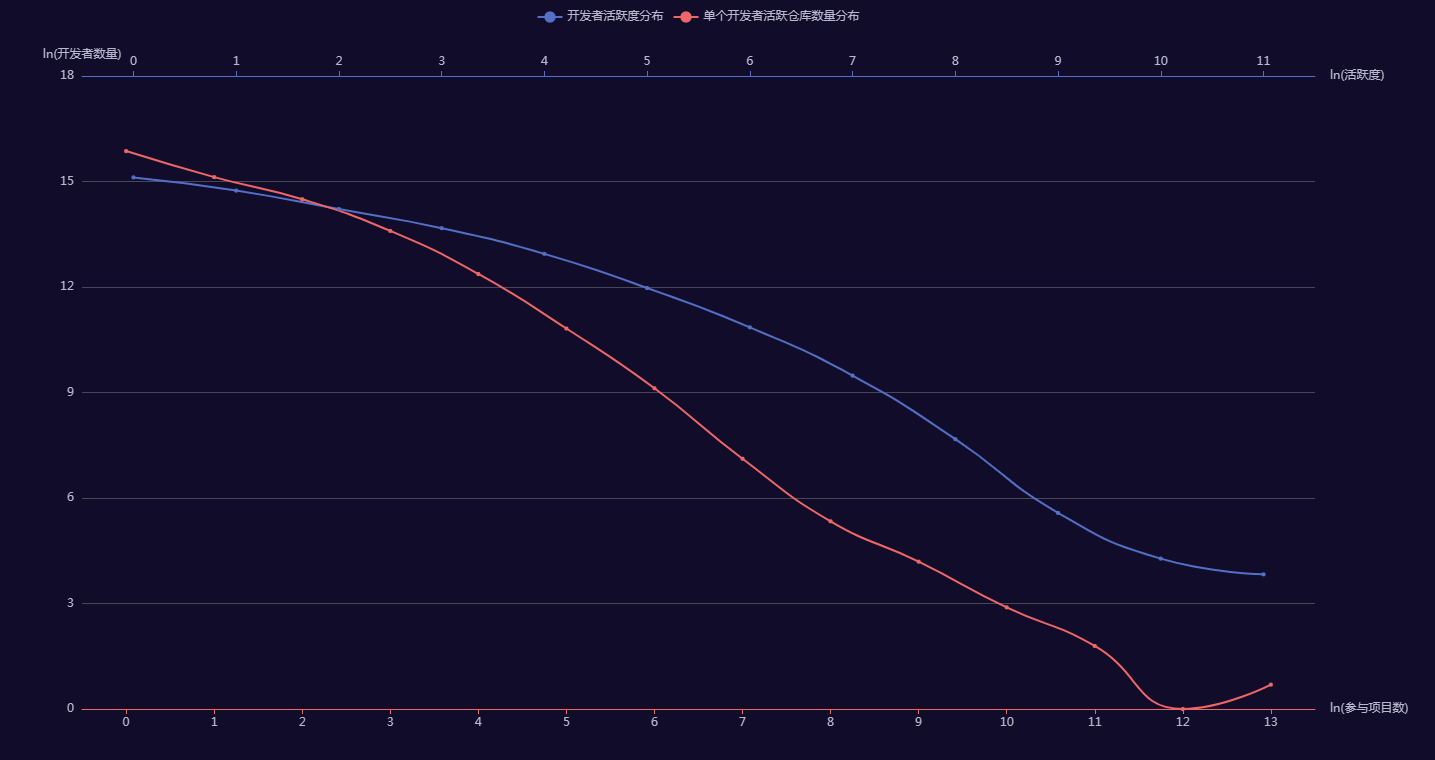
\includegraphics[width=130mm]{./figures/image2-1.png}
    \caption{开发者活跃度与活跃仓库数量分布图\\Figure 3-2: Distribution diagram of developer activity and the number of active warehouses}
\end{figure}

\par 图2-1使用双对数坐标系绘制,图上方的横坐标表示开发者活跃度,图下方横坐标表示开发者参与项目数量,纵坐标表示开发者数量,所谓双对数坐标,就是将原来的线性坐标轴都取自然对数,可以看到开发者活跃度与活跃仓库数量的分布符合幂律分布。经统计,活跃度超过 2,000 的开发者数量为 5,445 个,占全域开发者数量不足万分之六。而大部分开发者活跃度都在 [0, 500] 区间内,占全域开发者数量的 99.45\%,说明大多数开发者还是处于低活跃度的一个状态。观察曲线尾部,我们发现开发者活跃仓库数量在最后有一个回升,其实是由于部分未被过滤掉的自动化协作类账号的活跃仓库数量巨大,远超正常人类开发者,因此尾部形成V形曲线。





\subsubsection{个人发展}
% 语言使用分布;
% ​个人关注点(issue label讨论词云图);



\subsubsection{协作关系}
% 开发者协作网络;
% 项目关联网络;

\subsection{项目分析方法}
\subsubsection{项目生命力}
% 每日活跃度;
% 每日参与度;
% 项目回应度基于每日issue和pr的初次响应时间;

\subsubsection{项目多元化}
% 项目的时区特征;
% 项目国际化;
% 组织多元化

\subsubsection{协作的力量}
% 开发者协作网络;
% 关联项目网络;

\subsection{社区分析方法}
\subsubsection{开源象限}
% 影响力、全球化、社区规模

